\documentclass[aspectratio=169,11pt]{beamer}

\usetheme{default}
\usefonttheme{professionalfonts}
\usepackage[T1]{fontenc}
\usepackage{lmodern}
\usepackage{amsmath}
\usepackage{graphicx}

\definecolor{accent}{RGB}{0.40,0.07,0.07}
\setbeamercolor{frametitle}{fg=accent}
\setbeamercolor{title}{fg=accent}
\setbeamercolor{structure}{fg=accent}
\setbeamercolor{section in toc}{fg=accent}
\setbeamerfont{frametitle}{series=\bfseries}
\setbeamertemplate{navigation symbols}{}
\setbeamertemplate{footline}[frame number]
\setbeamertemplate{itemize items}[circle]
\setbeamertemplate{caption}{\centering\insertcaption\par}
\setbeamerfont{caption}{size=\footnotesize}
\setbeamerfont{title}{size=\Huge,series=\bfseries}
\setbeamerfont{subtitle}{size=\Large}

% Section divider slide
\AtBeginSection[]{
  \begin{frame}[plain]
    \vfill\centering
    {\usebeamercolor[fg]{title}\LARGE\bfseries\insertsectionhead\par}
    \vfill
  \end{frame}
}

% Image with a small label underneath, used in side-by-side figure rows
\newcommand{\labeledimg}[3]{%
  \begin{minipage}[t]{#1}\centering
    \includegraphics[height=#2]{#3}\par\vspace{2pt}
}
\newcommand{\imglabel}[1]{{\footnotesize #1}\end{minipage}}

\title{Analysis of the Obstacle Potential Function}
\author{}
\date{}

\begin{document}

\begin{frame}[plain]
  \titlepage
\end{frame}



% =====================================================================
\section{Cuurent Obtsacle Potential Function}

\begin{frame}{Obstacle potential}
  \[
    U_{obst} = \frac{\lambda\,(|\Delta v| / \Delta v_{max})}
                    {k(\Delta x, \Delta y, \Delta v_x, \Delta v_y)}
  \]
  \vspace{-0.5em}
  {\small
  \[
    k =
    \begin{cases}
      0, & |\Delta y| < l \text{ and } |\Delta x| < w \\[4pt]
      \left(1 - \dfrac{w}{|\Delta x|}\right)
        \sqrt{\left(\dfrac{\Delta x}{\tau(\Delta x, \Delta v_x)}\right)^2
            + \left(\dfrac{\Delta y}{\tau(\Delta y, \Delta v_y)}\right)^2},
        & |\Delta y| \leq \dfrac{l\,|\Delta x|}{w} \\[10pt]
      \left(1 - \dfrac{l}{|\Delta y|}\right)
        \sqrt{\left(\dfrac{\Delta x}{\tau(\Delta x, \Delta v_x)}\right)^2
            + \left(\dfrac{\Delta y}{\tau(\Delta y, \Delta v_y)}\right)^2},
        & \text{otherwise}
    \end{cases}
  \]}
  \vspace{-0.5em}
  {\small
  \begin{align*}
    \tau(\Delta x, \Delta v_x) &= \tfrac{1}{2}\Big[(1 + \alpha |\Delta v_x|)
      + (\alpha |\Delta v_x| - 1)\tanh(-\Delta x \Delta v_x)\Big]\,\tau_x \\
    \tau(\Delta y, \Delta v_y) &= \tfrac{1}{2}\Big[(1 + \alpha |\Delta v_y|)
      + (\alpha |\Delta v_y| - 1)\tanh(-\Delta y \Delta v_y)\Big]\,\tau_y
  \end{align*}}
  \vspace{-0.8em}
  {\footnotesize $\Delta x, \Delta y$: position relative to the obstacle vehicle;
  $\Delta v_x, \Delta v_y$: velocity relative to the obstacle vehicle.}
\end{frame}

\begin{frame}{Potential field $U_{obst}$}
  \centering
  \labeledimg{0.32\textwidth}{0.72\textheight}{potential_vx.png}
    \imglabel{Varying $\Delta v_x$}\hfill
  \labeledimg{0.32\textwidth}{0.72\textheight}{potential_vy.png}
    \imglabel{Varying $\Delta v_y$}\hfill
  \labeledimg{0.32\textwidth}{0.72\textheight}{potential_vxvy.png}
    \imglabel{Varying $\Delta v_x, \Delta v_y$}
\end{frame}

\begin{frame}{Force field $F = -\nabla U_{obst}$}
  \centering
  \labeledimg{0.32\textwidth}{0.72\textheight}{force_vx.png}
    \imglabel{Varying $\Delta v_x$}\hfill
  \labeledimg{0.32\textwidth}{0.72\textheight}{force_vy.png}
    \imglabel{Varying $\Delta v_y$}\hfill
  \labeledimg{0.32\textwidth}{0.72\textheight}{force_vxvy.png}
    \imglabel{Varying $\Delta v_x, \Delta v_y$}
\end{frame}

% =====================================================================
\section{Possible Issues}

\begin{frame}{Issue 1: Anomalous dip in force magnitude}
  \begin{columns}[c]
    \begin{column}{0.4\textwidth}
      \centering
      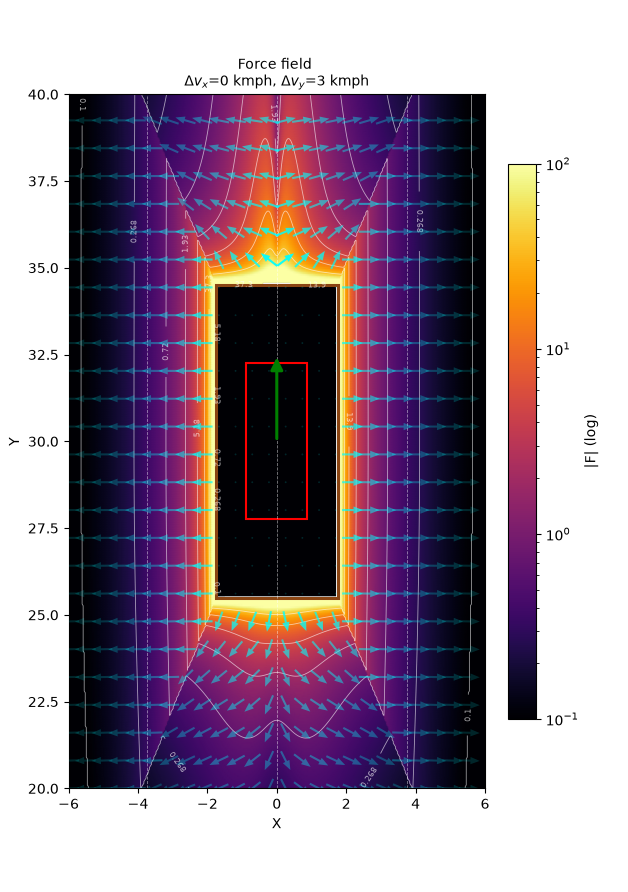
\includegraphics[height=0.78\textheight]{force_vy.png}
    \end{column}
    \begin{column}{0.55\textwidth}
      \begin{itemize}
        \item The force magnitude \textbf{dips near $x = 0$}.
        \item Undesirable: along $x = 0$ the force should be \emph{maximal}
              compared with neighbouring points.
      \end{itemize}
    \end{column}
  \end{columns}
\end{frame}

\begin{frame}{Issue 2: Sensitivity to $\tau_x, \tau_y$}
  \centering
  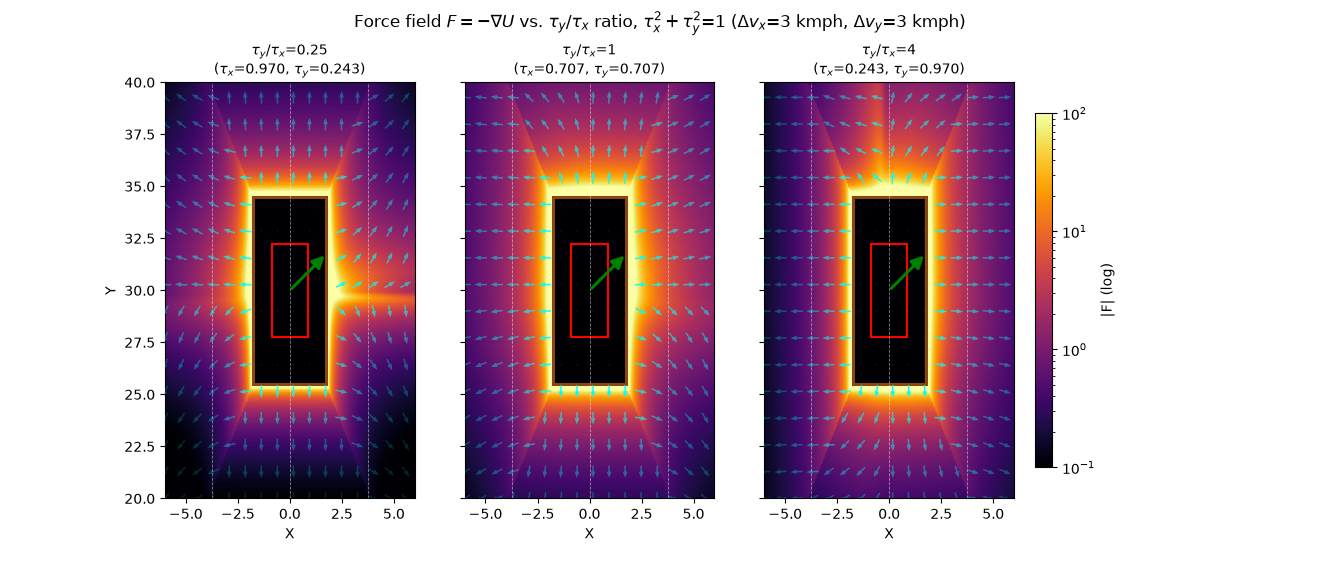
\includegraphics[width=0.92\textwidth]{tau_sensitivity.png}
  \vspace{0.5em}
  \begin{itemize}
    \item The shape of the potential is highly sensitive to $\tau_y/\tau_x$.
    \item Very large or very small ratios make the force field
          \textbf{parallel} in some regions.
  \end{itemize}
\end{frame}

\begin{frame}{Issue 3: Velocity behaviour at a fixed point}
  \begin{columns}[c]
    \begin{column}{0.55\textwidth}
      \centering
      
\includegraphics[width=\linewidth]{base_vel.png}
    \end{column}
    \begin{column}{0.42\textwidth}
      \begin{itemize}
        \item Force \textbf{increases} with receding velocity at a fixed point.
        \item Ideally the repulsive force should \textbf{decrease} when the
              vehicles are receding.
      \end{itemize}
    \end{column}
  \end{columns}
\end{frame}

\begin{frame}{Issue 4: More free parameters than DOF}
  \begin{itemize}
    \item The model has \textbf{4 free parameters}: $\lambda$, $\alpha$,
          $\tau_x$, $\tau_y$.
    \item The model only has \textbf{3 degrees of freedom}.
    \item Reducing the parameter count will help the optimisation problem.
  \end{itemize}
\end{frame}

% =====================================================================
\section{Potential Fixes}

\begin{frame}{Force dip: the cause}
  \begin{columns}[c]
    \begin{column}{0.58\textwidth}
      The dip comes from the skewed distance
      \[
        k = \sqrt{(x/\tau_x)^2 + (y/\tau_y)^2}
      \]
      \[
        U(k) = \frac{\lambda\,(|\Delta v| / \Delta v_{max})}{k},
        \qquad F = -\nabla U
      \]
      \[
        \nabla U = U'(k)\,\nabla k
        \quad\Rightarrow\quad
        |\nabla U| = |U'(k)|\cdot|\nabla k|
      \]
      $|\nabla k|$ is not uniform, which creates the dip.
    \end{column}
    \begin{column}{0.38\textwidth}
      \centering
      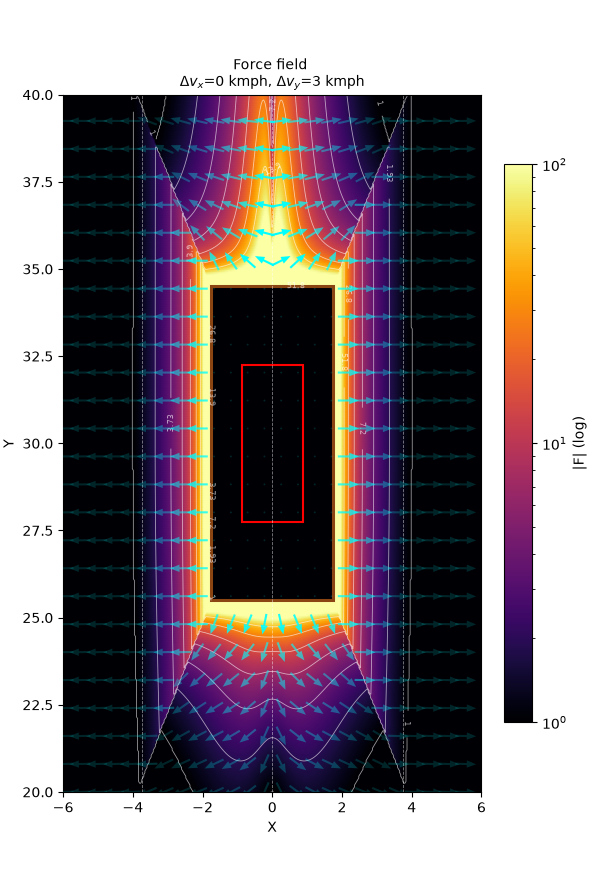
\includegraphics[height=0.75\textheight]{force_dip_before_fix.png}
    \end{column}
  \end{columns}
\end{frame}

\begin{frame}{Force dip: the cause}
  \centering
  \vfill
  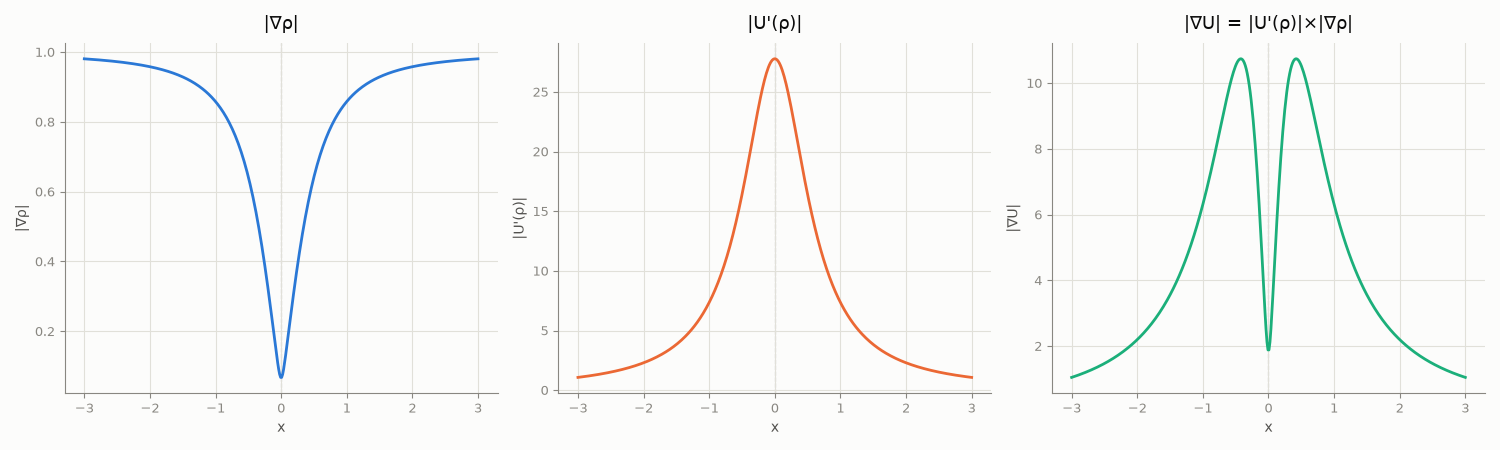
\includegraphics[width=\textwidth]{force_dip_cause.png}
  \vfill
  $|\nabla U| = |U'(k)|\cdot|\nabla k|$
  \vfill
\end{frame}

\begin{frame}{Force dip: the fix}
  \begin{columns}[c]
    \begin{column}{0.55\textwidth}
      \[
        U'(k) = -\frac{\lambda\,(|\Delta v| / \Delta v_{max})}{k^{2}}
      \]
      $U'(k)$ falls off smoothly with $k$ and has no dip or ridge of its own.

      \medskip
      Normalise the gradient direction:
      \[
        F = -\frac{\nabla U}{|\nabla k|} = -U'(k)\,\frac{\nabla k}{|\nabla k|},
        \qquad |F| = |U'(k)|
      \]
    \end{column}
    \begin{column}{0.42\textwidth}
      \centering
      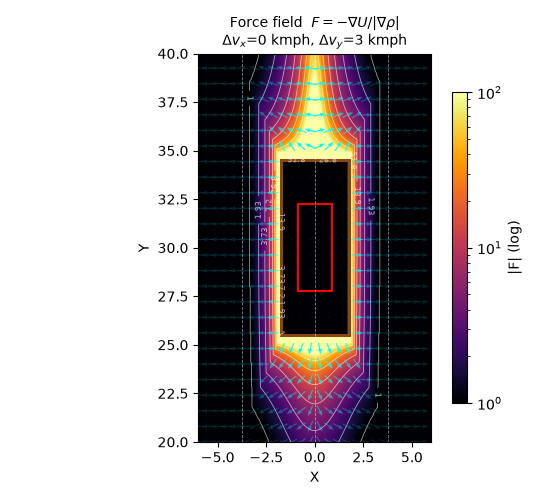
\includegraphics[width=\linewidth]{force_dip_after_fix.png}
    \end{column}
  \end{columns}
\end{frame}

\begin{frame}{$\tau$ sensitivity: the cause}
  {\small
  \[
    U = \frac{\lambda(\Delta v/v)}{k}
  \]
  \vspace{-1.2em}
  \[
    k =
    \begin{cases}
      0, & |\Delta y| < l \text{ and } |\Delta x| < w \\[4pt]
      \left(1-\dfrac{w}{|\Delta x|}\right)
        \sqrt{\left(\dfrac{\Delta x}{\tau(\Delta x,\Delta v_x)}\right)^2
            + \left(\dfrac{\Delta y}{\tau(\Delta y,\Delta v_y)}\right)^2},
        & |\Delta y| \le \dfrac{l|\Delta x|}{w} \\[10pt]
      \left(1-\dfrac{l}{|\Delta y|}\right)
        \sqrt{\left(\dfrac{\Delta x}{\tau_x}\right)^2
            + \left(\dfrac{\Delta y}{\tau_y}\right)^2},
        & \text{otherwise}
    \end{cases}
  \]}
  \begin{itemize}
    \item If $\tau_y \ll \tau_x$, the $y^2/\tau_y^2$ term dominates.
    \item The potential then does not change across $x$ $\Rightarrow$
          \textbf{no lateral force} in the forward and backward regions.
    \item The same happens in the side region when $\tau_y/\tau_x \gg 1$.
  \end{itemize}
\end{frame}

\begin{frame}{$\tau$ sensitivity: the fix}
  $k$ already splits space into regions, so use \textbf{different $\tau$ per region}:
  {\small
  \[
    K =
    \begin{cases}
      0, & |\Delta y| < l \text{ and } |\Delta x| < w \\[4pt]
      \left(1-\dfrac{w}{|\Delta x|}\right)
        \sqrt{\left(\dfrac{\Delta x}{\tau(\Delta x,\Delta v_x,\tau_2)}\right)^2
            + \left(\dfrac{\Delta y}{\tau(\Delta y,\Delta v_y,\tau_1)}\right)^2},
        & |\Delta y| \le \dfrac{l|\Delta x|}{w} \\[10pt]
      \left(1-\dfrac{l}{|\Delta y|}\right)
        \sqrt{\left(\dfrac{\Delta x}{\tau(\Delta x,\Delta v_x,\tau_1)}\right)^2
            + \left(\dfrac{\Delta y}{\tau(\Delta y,\Delta v_y,\tau_2)}\right)^2},
        & \text{otherwise}
    \end{cases}
  \]
  \[
    \tau(\Delta x, \Delta v_x, \tau) = \frac{\tau}{2}\Big[(1+\alpha|\Delta v_x|)
      + (\alpha|\Delta v_x|-1)\tanh(-\Delta x \Delta v_x)\Big]
  \]}
\end{frame}

\begin{frame}{$\tau$ sensitivity: comparison}
  \centering
  \labeledimg{0.45\textwidth}{0.74\textheight}{force_tau_before_fix.png}
    \imglabel{Before: $\tau_y/\tau_x > 5$}\hfill
  \labeledimg{0.45\textwidth}{0.74\textheight}{force_tau_after_fix.png}
    \imglabel{After: $\tau_2/\tau_1 > 5$}
\end{frame}

\begin{frame}{Velocity behaviour: the issue}
  \begin{columns}[c]
    \begin{column}{0.5\textwidth}
      \centering
      
\includegraphics[width=0.9\linewidth]{base_vel.png}\par
      {\footnotesize Original}
    \end{column}
    \begin{column}{0.5\textwidth}
      \centering
      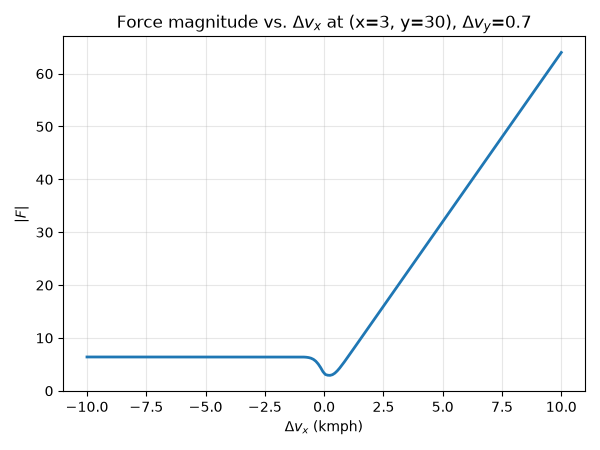
\includegraphics[width=0.9\linewidth]{vel_original.png}\par
      {\footnotesize After removing $|\Delta v|/\Delta v_{max}$}
    \end{column}
  \end{columns}
  \medskip
  \begin{itemize}
    \item Force grows with receding velocity because of the
          $|\Delta v|/\Delta v_{max}$ term in the numerator.
    \item Fix is to remove that term, $\;U(k) = \lambda / k$.
    \item The remaining kink comes from the $\tau$ term.
  \end{itemize}
\end{frame}

\begin{frame}{Reformulating $\tau$}
  Current form:
  \[
    \tau = \Big[(1+\alpha|\Delta v_x|) + (\alpha|\Delta v_x|-1)
           \tanh(-\Delta x \Delta v_x)\Big]\,\tau_x
  \]
  Original goal:
  \[
    \tau = \tau_x \ \text{(receding)}, \qquad
    \tau = \alpha\tau_x|\Delta v_x| \ \text{(approaching)}
  \]
  Better: $\tau$ should be larger when vehicles approach:
  \[
    \tau = \tau_x \ \text{(receding)}, \qquad
    \tau = \tau_x(1+\alpha|\Delta v_x|) \ \text{(approaching)}
  \]
\end{frame}

\begin{frame}{Formulation 1}
  {\small
  \[
    \tau = \Big[\big(1+(1+\alpha|\Delta v_x|)\big)
      + \big((1+\alpha|\Delta v_x|)-1\big)\tanh(-\Delta x \Delta v_x)\Big]\,\tau_x
  \]}
  \begin{columns}[c]
    \begin{column}{0.55\textwidth}
      \centering
      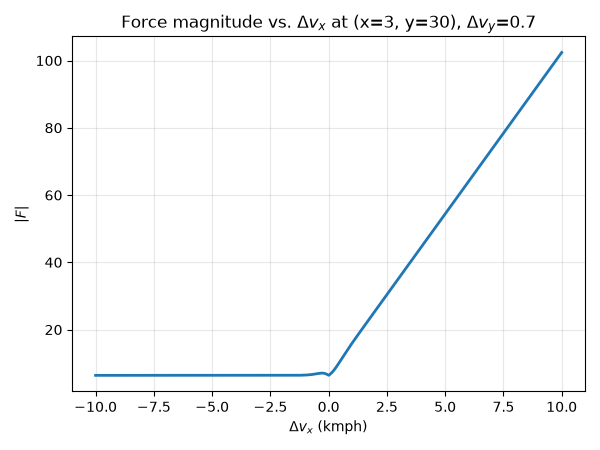
\includegraphics[width=\linewidth]{vel_formulation1.png}
    \end{column}
    \begin{column}{0.42\textwidth}
      \begin{itemize}
        \item Force magnitude vs.\ $\Delta v_x$.
        \item We still want the repulsive force to \textbf{decrease} with
              increasing receding velocity.
      \end{itemize}
    \end{column}
  \end{columns}
\end{frame}

\begin{frame}{Formulation 2}
  {\small
  \[
    \tau = \Big[\Big(\tfrac{1}{1+\alpha|\Delta v_x|}+(1+\alpha|\Delta v_x|)\Big)
      + \Big((1+\alpha|\Delta v_x|)-\tfrac{1}{1+\alpha|\Delta v_x|}\Big)
        \tanh(-\Delta x \Delta v_x)\Big]\,\tau_x
  \]}
  \begin{columns}[c]
    \begin{column}{0.55\textwidth}
      \centering
      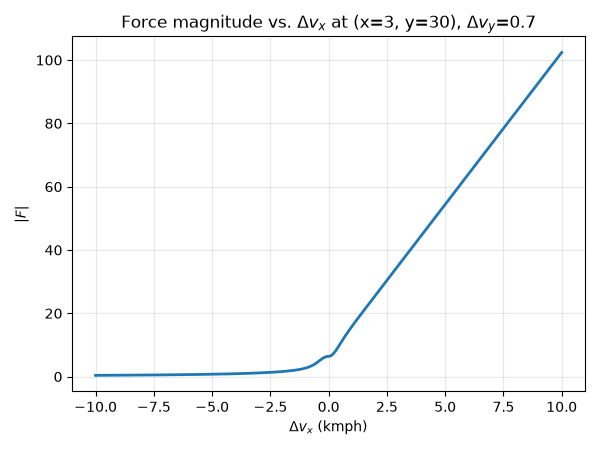
\includegraphics[width=\linewidth]{vel_formulation2.png}
    \end{column}
    \begin{column}{0.42\textwidth}
      \begin{itemize}
        \item For high approaching velocity,
              $\tau \approx \alpha|\Delta v_x|\,\tau_x$.
        \item $\alpha$ and $\tau_x$ become redundant.
        \item Use $\alpha$ instead to control the \textbf{power} of the
              velocity term.
      \end{itemize}
    \end{column}
  \end{columns}
\end{frame}

\begin{frame}{Formulation 3}
  {\small
  \[
    \tau = \Big[\Big(\tfrac{1}{(1+|\Delta v_x|)^{\alpha}}+(1+|\Delta v_x|)^{\alpha}\Big)
      + \Big((1+|\Delta v_x|^{\alpha})-\tfrac{1}{(1+|\Delta v_x|)^{\alpha}}\Big)
        \tanh(-\Delta x \Delta v_x)\Big]\,\tau_x
  \]}
  \centering
  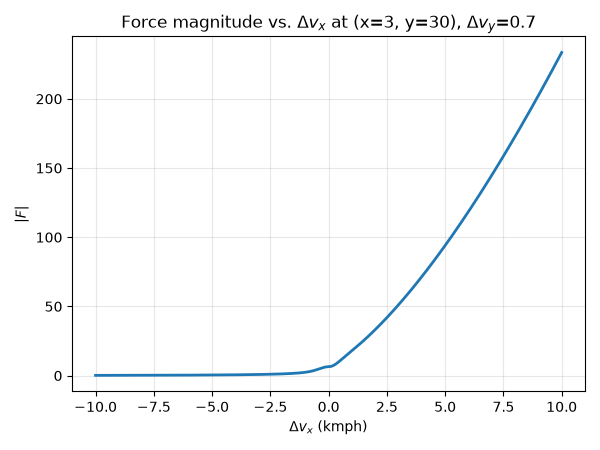
\includegraphics[height=0.62\textheight]{vel_formulation3.png}\par
  {\footnotesize Force magnitude vs.\ $\Delta v_x$ under Formulation 3}
\end{frame}

\begin{frame}{Formulations compared}
  \centering
  \labeledimg{0.32\textwidth}{0.72\textheight}{form_1.png}
    \imglabel{Formulation 1}\hfill
  \labeledimg{0.32\textwidth}{0.72\textheight}{form_2.png}
    \imglabel{Formulation 2}\hfill
  \labeledimg{0.32\textwidth}{0.72\textheight}{form_3.png}
    \imglabel{Formulation 3}
\end{frame}

\begin{frame}{Fix 4 --- Reducing free parameters}
  Define
  \[
    \gamma = \frac{\tau_y}{\tau_x}, \qquad \beta = \lambda \tau_x
  \]
  The equation reduces to
  {\small
  \[
    U = \frac{\beta(\Delta v/v)}{k}, \qquad
    k =
    \begin{cases}
      0, & |\Delta y| < l \text{ and } |\Delta x| < w \\[4pt]
      \left(1-\dfrac{w}{|\Delta x|}\right)
        \sqrt{(\Delta x)^2 + \left(\dfrac{\Delta y}{\tau(\gamma)}\right)^2},
        & |\Delta y| \le \dfrac{l|\Delta x|}{w} \\[10pt]
      \left(1-\dfrac{l}{|\Delta y|}\right)
        \sqrt{(\Delta x)^2 + \left(\dfrac{\Delta y}{\tau(\gamma)}\right)^2},
        & \text{otherwise}
    \end{cases}
  \]}
  \begin{itemize}
    \item Free parameters reduced from $\lambda, \tau_x, \tau_y$ to
          $\gamma, \beta$.
  \end{itemize}
\end{frame}

% =====================================================================
\section{Combining the changes}

\begin{frame}{Final combinations}
  \centering
  \labeledimg{0.32\textwidth}{0.72\textheight}{final_1.png}
    \imglabel{All modifications combined}\hfill
  \labeledimg{0.32\textwidth}{0.72\textheight}{final_2.png}
    \imglabel{Formulation 1}\hfill
  \labeledimg{0.32\textwidth}{0.72\textheight}{final_3.png}
    \imglabel{Formulation 1 without $\tau$ correction}
\end{frame}

\end{document}
